% !TEX root =  master.tex
\chapter{Proposed web application}\label{chapter:webapp}
\chapterauthor{Written by Tobias Richstein}

Since we do not plan to hand in a sample notebook to the Kaeggle challenge, we decided to build some sort of application that makes the result of our work a little more accessible and easily usable. In the end we settled on providing access to the models via a website that runs inference on the backend. We settled on using the framework \textit{Flask} \autocite{ronacher_flask_nodate} since it uses Python just as the rest of the project.

The interface which can be seen in figure \vref{fig:app} is very simple but functional and built with the templating engine \textit{Jinja 2} that is included with Flask. The user can first upload an image that is then previewed before choosing which model configuration to run: Faster \ac{R-CNN}, \ac{YOLO} or the ensemble of both. When clicking the submit button inference is run on the backend with the selected bounding box model as well as the study level model and the result is returned by re-rendering the webpage with the bounding boxes that were predicted. Their scores and coordinates also appear alongside the image. The output of the study level model is shown as well by the scores for the individual classes. The highest score is the one that the model has predicted.

We also provide a Dockerfile to containerize the entire application including the models to easily be able to build and run our results anywhere. Additionally a prebuilt Docker image is available on Docker Hub and can be run with: \texttt{docker run -p 5000:5000 tobiasrst/aml-project:latest}. The app will then be available on the host on port 5000. Using the sample image located in the project directory at \texttt{/src/app/example.png} the inference can be tested quickly.

\begin{figure*}[]
	\centering
	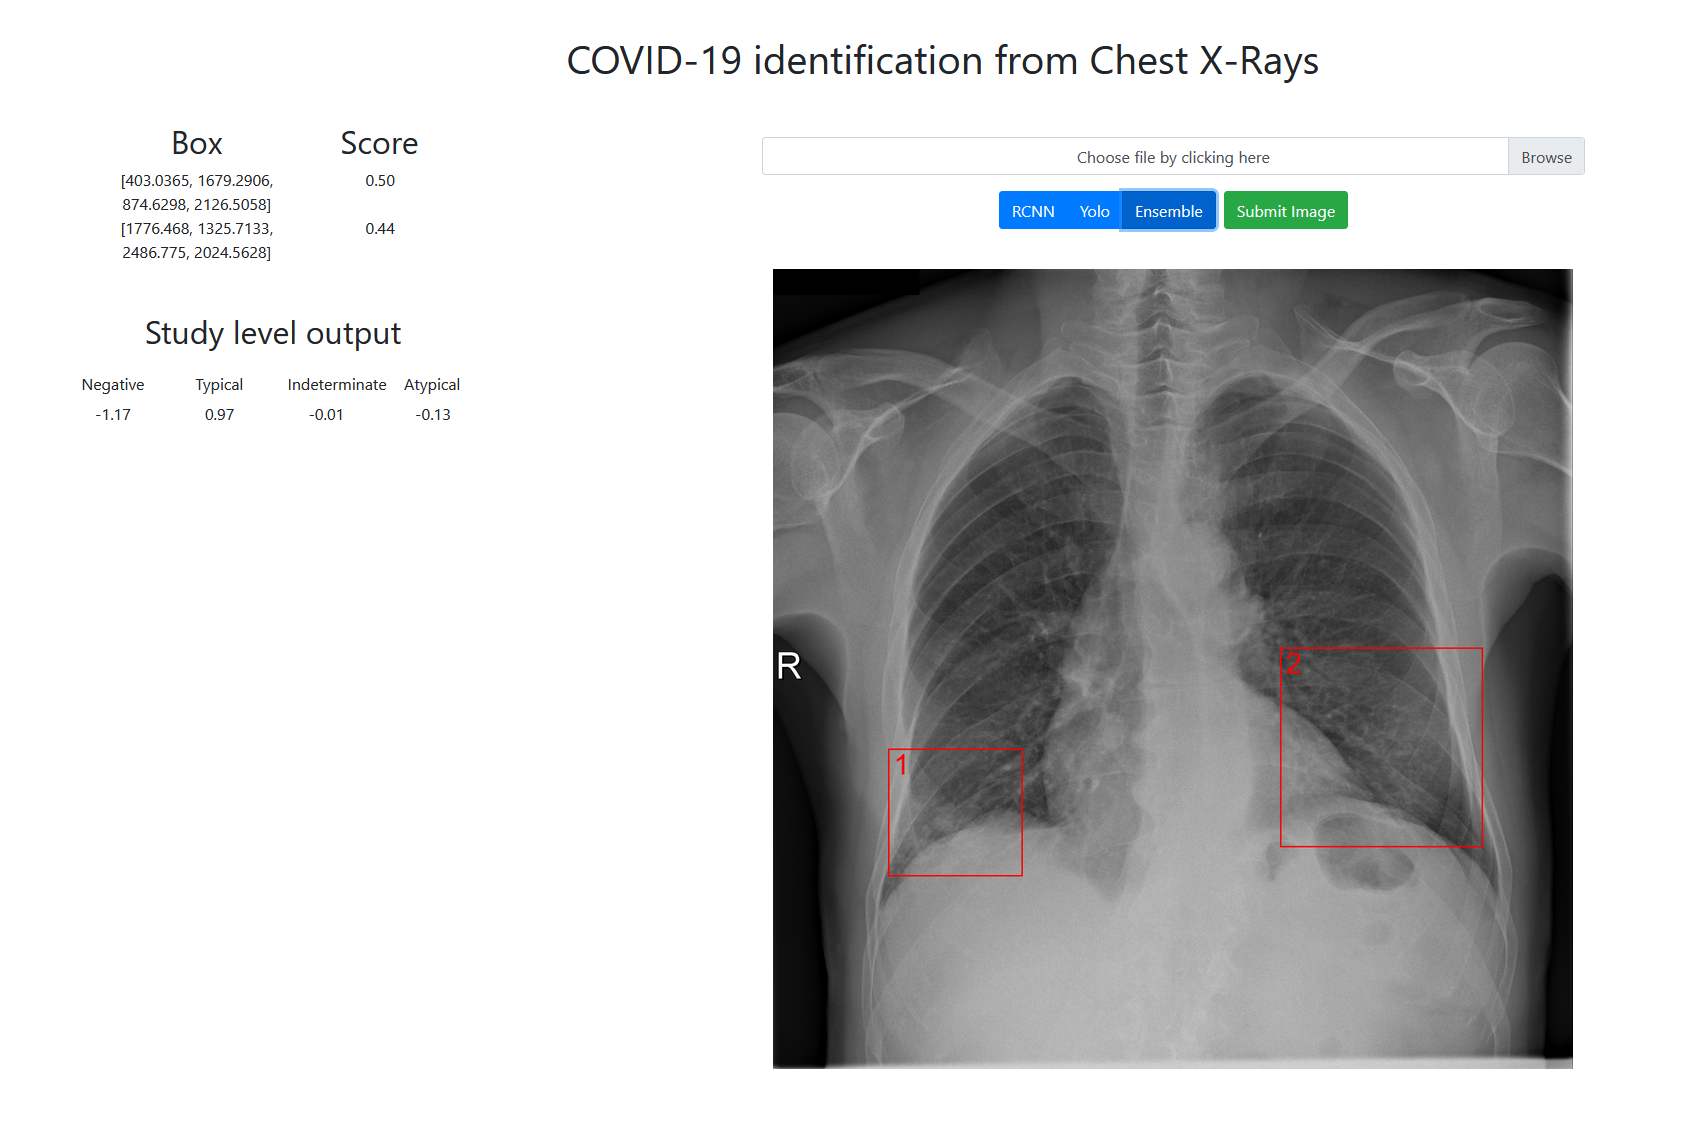
\includegraphics[width=0.9\linewidth]{img/app.png}
	\caption{The web-app interface with a returned result}
	\label{fig:app}
\end{figure*}